\documentclass[12pt]{article}
\usepackage{fancyvrb}
\usepackage{graphicx}
\usepackage{url}
\usepackage{comment}
\usepackage{pgf}
\usepackage{wasysym}

\usepackage{geometry}
\usepackage{multicol}
\usepackage{relsize}
\usepackage{xcolor}
\usepackage{hyperref}
\usepackage{tabu}
\usepackage{longtable,booktabs}

\geometry{
  %includeheadfoot,
  margin=2.54cm
}

\fvset{tabsize=2}
\fvset{fontsize=\relsize{-1}}
\fvset{frame=single}

\title{Creating RESTful APIs with NodeJS and MongoDB Tutorial}
\author{}
\date{}

\begin{document}
\maketitle

This exercise is about creating a RESTful API using Node.js (Express.js)
and MongoDB (mongoose)! You will learn how to install and use
each component individually and then proceed to create a RESTful API.

\section{What is a RESTful API?}

REST stands for Representational State Transfer. It is an architecture
that allows \texttt{client-server} communication through a uniform
interface. REST is \emph{stateless}, \emph{cachable} and has
property called \emph{idempotence}; the side effect of
identical requests have the same side-effect as a single request.

HTTP RESTful API's are composed of:
\begin{description}
\item[HTTP methods] --- e.g., GET, PUT, DELETE, PATCH, POST, \ldots{}
\item[Base URI] --- e.g., \texttt{http://www.dcs.bbk.ac.uk}
\item[URL path] --- e.g., \texttt{/path/creating-a-restful-api-tutorial-with-nodejs-and-mongodb/}
\item[Media type] --- e.g., \texttt{html}, \texttt{JSON}, \texttt{XML},
  \texttt{Microformats}, \texttt{Atom}, \texttt{Images}, \ldots{}
\end{description}

\noindent Here is a summary what we want to implement:
\begin{longtable}[]{@{}lllll@{}}
\toprule
Resource (URI) & POST (create) & GET (read) & PUT (update) & DELETE
(destroy)\tabularnewline
\midrule
\endhead
/todos & create new task & list tasks & N/A (update all) & N/A (destroy
all)\tabularnewline
/todos/1 & error & show task ID 1 & update task ID 1 & destroy task ID
1\tabularnewline
\bottomrule
\end{longtable}
\textbf{NOTE} for this tutorial:
\begin{itemize}
\item
  The format will be JSON.
\item
  Bulk updates and bulk destroys are not safe, so we will not be implementing those.
\item
  \textbf{CRUD} functionality: POST == \textbf{C}REATE, GET ==
  \textbf{R}EAD, PUT == \textbf{U}PDATE, DELETE == \textbf{D}ELETE.
\end{itemize}

\section{Installing the MEAN Stack backend}

In this section, we are going to install the main backend components of the
MEAN stack: MongoDB, NodeJS and ExpressJS.

\subsection{Installing MongoDB}

MongoDB is a document-oriented NoSQL database (Big Data ready). It
stores data in JSON-like format and allows users to perform SQL-like
queries against it.

You can install MongoDB following these
\href{http://docs.mongodb.org/manual/installation/}{instructions}.

If you have a \textbf{Mac} and \href{http://brew.sh/}{brew} it's just:
\begin{Verbatim}
brew install mongodb && mongod
\end{Verbatim}

In \textbf{Ubuntu}:
\begin{Verbatim}
sudo apt-get -y install mongodb
\end{Verbatim}

In Windows you need to simply double-click the downloaded \verb!msi! file.

After you have installed MongoDB you should then check the version:
\begin{Verbatim}
mongod --version

# => db version v2.6.4
# => 2014-10-01T19:07:26.649-0400 git version: nogitversion
\end{Verbatim}

\subsection{Installing NodeJS}

The Node official description is:
\begin{quote}
Node.js is a JavaScript runtime built on Chrome's V8 JavaScript engine.
Node.js uses an event-driven, non-blocking I/O model that makes it
lightweight and efficient. Node.js' package ecosystem, npm, is the
largest ecosystem of open source libraries in the world.

\textbf{Node.js Website}\href{https://nodejs.org}{nodejs.org}
\end{quote}
In short, NodeJS allows you to run Javascript outside the browser, in
this case, on the web server. NPM allows you to install/publish node
packages with ease.

To install it, you can go to the \href{http://nodejs.org/}{NodeJS Website}.

Since Node versions changes very often. You can use the NVM (Node
Version Manager) with:
\begin{Verbatim}
# *nix version - Windows is slightly different (see the distribution download page for details)
# download NPM
curl -o- https://raw.githubusercontent.com/creationix/nvm/v0.31.4/install.sh | bash

# load NPM
export NVM_DIR="$HOME/.nvm"
[ -s "$NVM_DIR/nvm.sh" ] && . "$NVM_DIR/nvm.sh" # This loads nvm

# Install latest stable version
nvm install stable
\end{Verbatim}
Check out \url{https://github.com/creationix/nvm} for more details.

On the \textbf{Mac} with \href{http://brew.sh}{Homebrew} you can do:
\begin{Verbatim}
brew install nodejs
\end{Verbatim}
After you have it installed, check the version of node and npm (node package
manager):
\begin{Verbatim}
node -v
# => v6.2.2
npm -v
# => 3.9.5
\end{Verbatim}
or something similar.

\subsection{Installing ExpressJS}

ExpressJS is a web application framework that runs on NodeJS. It allows
you to build web applications and API endpoints. (more details on this later).

We are going to create a project folder \verb!first!, and then add
\texttt{express} as a dependency. Let's use NPM init command to get us
started.
\begin{Verbatim}
# create project folder
mkdir todo-app

# move to the folder and initialise the project
cd todo-app
npm init .  

# press enter multiple times to accept all defaults
# install express and save it as dependency
npm install express --save
\end{Verbatim}
Notice that after the last command, \texttt{express} should be added to
\verb!package.json! with the version the appropriate version information.

\section{Using MongoDB with Mongoose}

Mongoose is an NPM package that allows you to interact with MongoDB. You
can install it as follows:
\begin{Verbatim}
npm install mongoose --save
\end{Verbatim}
If you followed the previous steps, you should have all the software you need to
complete this tutorial. We are going to build an API that allow users to
CRUD (Create-Read-Update-Delete) Todo tasks from a database.

\subsection{Mongoose CRUD}

CRUD == \textbf{C}reate-\textbf{R}ead-\textbf{U}pdate-\textbf{D}elete

We are going to create, read, update and delete data from MongoDB using
Mongoose/Node. First, you need to have \verb!mongodb! up and running:
\begin{Verbatim}
# run mongo daemon
mongod
\end{Verbatim}
Keep mongo running in a terminal window and while in the folder
\texttt{todoApp} type \texttt{node} to enter the node command line interpreter (CLI). Then type:
\begin{Verbatim}
// Load mongoose package
var mongoose = require('mongoose');

// Connect to MongoDB and create/use database called todoApp
mongoose.connect('mongodb://localhost/todoApp');

// Create a schema
var TodoSchema = new mongoose.Schema({  
	name: String,  
	completed: Boolean,  
	note: String,  
	updated_at: { type: Date, default: Date.now }
});

// Create a model based on the schema
var Todo = mongoose.model('Todo', TodoSchema);
\end{Verbatim}
Now, let's test that we can save and edit data.

\subsection{Mongoose Create}

\begin{Verbatim}
// Create a todo in memory
var todo = new Todo({name: 'Master NodeJS', completed: false, 
	note: 'Getting there...'});

// Save it to the database
todo.save(function(err){  
	if(err)    
		console.log(err);  
	else    
		console.log(todo);
});
\end{Verbatim}
If you take a look at Mongo you will notice that we just created an
entry. You can easily visualise the data using a tool such as 
\href{https://robomongo.org/}{Robomongo}.

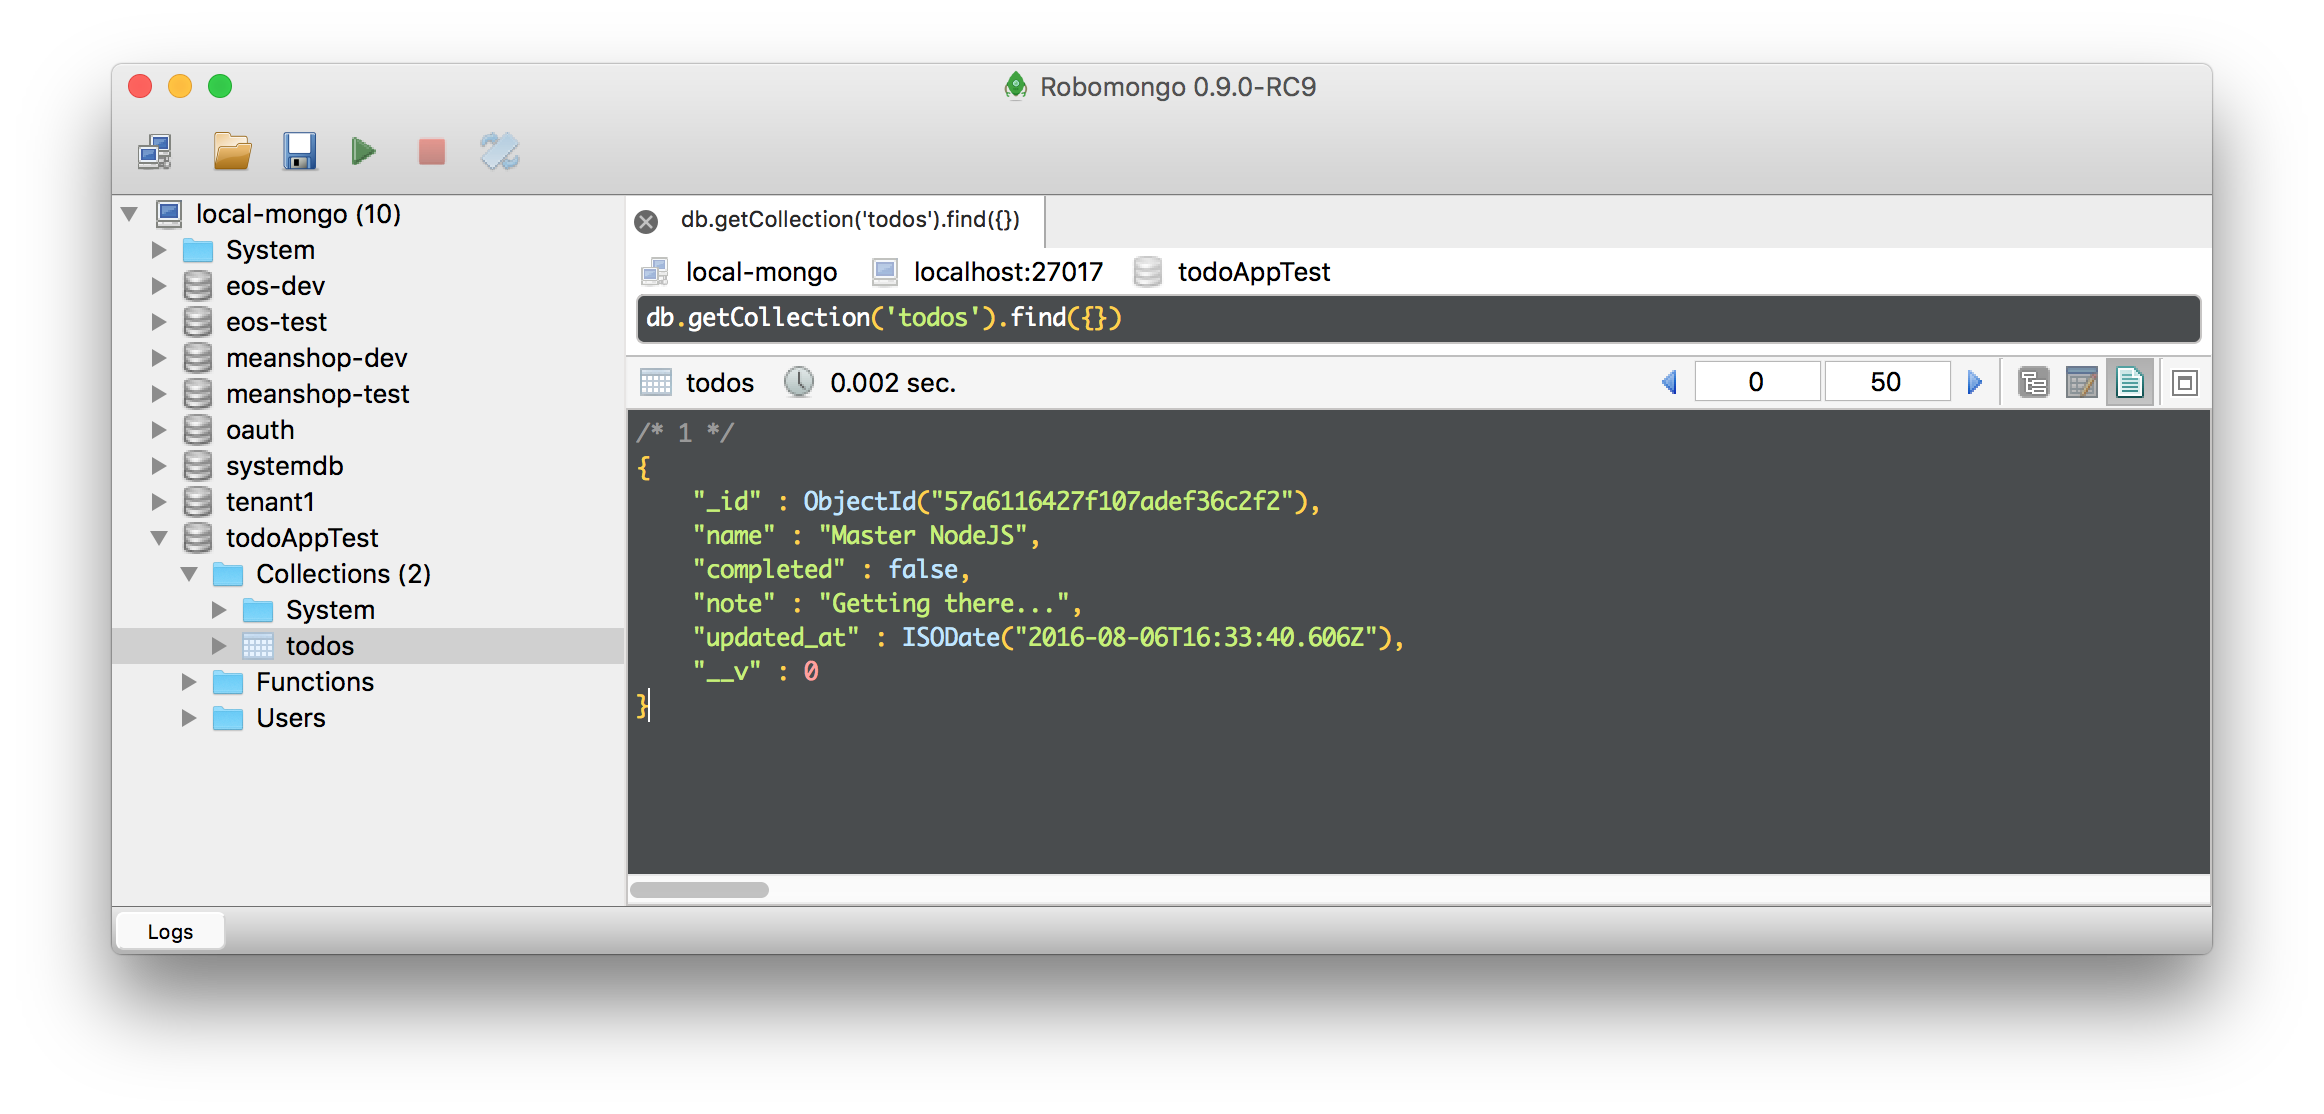
\includegraphics[width=\textwidth]{images/robomongo}

You can also build the object and save it in one step using
\texttt{create}:
\begin{Verbatim}
Todo.create({name: 'Create something with Mongoose', completed: true, 
	note: 'this is one'}, function(err, todo){  
		if(err) console.log(err);  
		else console.log(todo);
});
\end{Verbatim}

\subsection{Mongoose Read and Query}

So far we have been able to save data, now we are going explore how to
query the information. There are multiple options for reading/querying
data:

\begin{itemize}
\item
  \verb!Model.find(conditions, {[}fields{]}, {[}options{]}, {[}callback{]})!
\item
  \verb!Model.findById(id, {[}fields{]}, {[}options{]}, {[}callback{]})!
\item
  \verb!Model.findOne(conditions, {[}fields{]}, {[}options{]}, {[}callback{]})!
\end{itemize}
Some examples:
\begin{Verbatim}
// Find all data in the Todo collection
Todo.find(function (err, todos) {  
	if (err) return console.error(err);  
	console.log(todos)
});
\end{Verbatim}
The result is something like this:
\begin{Verbatim}
[ { _id: 57a6116427f107adef36c2f2,    
	name: 'Master NodeJS',    
	completed: false,    
	note: 'Getting there...',    
	__v: 0,    
	updated_at: 2016-08-06T16:33:40.606Z },  
  { _id: 57a6142127f107adef36c2f3,    
	name: 'Create something with Mongoose',    
	completed: true,    
	note: 'this is one',    __v: 0,    
	updated_at: 2016-08-06T16:45:21.143Z } ]
\end{Verbatim}
You can also add queries:
\begin{Verbatim}
// callback function to avoid duplicating it all over
var callback = function (err, data) {  
	if (err) { return console.error(err); }  
	else { console.log(data); }}
	
	// Get ONLY completed tasks
	Todo.find({completed: true }, callback);
	
	// Get all tasks ending with `JS`
	Todo.find({name: /JS$/ }, callback);
\end{Verbatim}
You can chain multiple queries, e.g.:
\begin{Verbatim}
var oneYearAgo = new Date();
oneYearAgo.setYear(oneYearAgo.getFullYear() - 1);

// Get all tasks staring with `Master`, completed
Todo.find({name: /^Master/, completed: true }, callback);

// Get all tasks staring with `Master`, not completed and created within the last year
Todo.find({name: /^Master/, completed: false })
	.where('updated_at')
	.gt(oneYearAgo)
	.exec(callback);
\end{Verbatim}
The MongoDB query language is very powerful. We can combine regular
expressions, date comparison and more.

\subsection{Mongoose Update}

Moving on, we are now going to explore how to update data.

Each model has an \texttt{update} method which accepts multiple updates
(for batch updates, because it doesn't return an array with data).
\begin{itemize}
\item
  \verb!Model.update(conditions, update, {[}options{]}, {[}callback{]})!
\item
  \verb!Model.findByIdAndUpdate(id, {[}update{]}, {[}options{]}, {[}callback{]})!
\item
\begin{verbatim}
  Model.findOneAndUpdate({[}conditions{]}, {[}update{]}, {[}options{]}, 
  			{[}callback{]})
\end{verbatim}
\end{itemize}
Alternatively, the method \texttt{findOneAndUpdate} could be used to
update just one and return an object.
\begin{Verbatim}
// Model.update(conditions, update, [options], [callback])
// update `multiple tasks from complete false to true

Todo.update({ name: /master/i }, { completed: true }, { multi: true }, callback);

//Model.findOneAndUpdate([conditions], [update], [options], [callback])
Todo.findOneAndUpdate({name: /JS$/ }, {completed: false}, callback);
\end{Verbatim}
As you might have noticed the batch updates (\texttt{multi:\ true}) doesn't
show the data, but instead displays the number of fields that were modified.
\begin{Verbatim}
{ ok: 1, nModified: 1, n: 1 }
\end{Verbatim}
Here is what those fields mean:
\begin{itemize}
\item
  \texttt{n} means the number of records that matches the query
\item
  \texttt{nModified} represents the number of documents that were
  modified with update query.
\end{itemize}

\subsection{Mongoose Delete}

\texttt{update} and \texttt{remove} mongoose API are identical, the only
difference it is that no elements are returned. Try it on your own ;)

\begin{itemize}
\item
  \verb!Model.remove(conditions, {[}callback{]})!
\item
  \verb!Model.findByIdAndRemove(id, {[}options{]}, {[}callback{]})!
\item
  \verb!Model.findOneAndRemove(conditions, {[}options{]}, {[}callback{]})!
\end{itemize}

\section{ExpressJS and Middleware}

ExpressJS is a complete web framework solution. It has HTML template
solutions (jade, ejs, handlebars, hogan.js) and CSS pre-compilers (less,
stylus, compass). Through middleware layers, it handles: cookies,
sessions, caching, Cross-Site Request Forgery (CSRF), compression, and much more.

\textbf{Middleware} in this context are pluggable processors that runs on each request
made to the server. You can have any number of middleware that will
process the request one by one in a serial fashion. Some middleware
might alter the request input. Others, might create log outputs, add
data and pass it to the \texttt{next()} middleware in the chain.

We can use the middleware using \texttt{app.use}. That will apply for
all request. If you want to be more specific, you can use
\texttt{app.}\emph{verb}. For instance: \verb!app.get!, \verb!app.delete!, 
\verb!app.post!, \verb!app.update!, \ldots{}

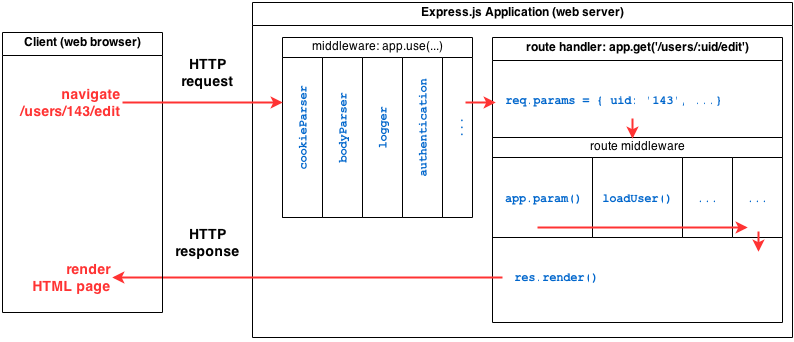
\includegraphics[width=\textwidth]{images/express-middleware}

Here are some examples of middleware layers to illustrate this point.

Say you want to log the IP of the client on each request:
\begin{Verbatim}
app.use(function (req, res, next) {  
	var ip = req.headers['x-forwarded-for'] || req.connection.remoteAddress;  
	console.log('Client IP:', ip);  next();
});
\end{Verbatim}
Notice that each middleware layer has three parameters:
\begin{itemize}
\item
  \texttt{req}: contain all the requests objects like URLs, path,
  \ldots{}
\item
  \texttt{res}: is the response object where we can send the reply back
  to the client.
\item
  \texttt{next}: continue with the next middleware in the chain.
\end{itemize}
You can also specify a path that you want the middleware to activate on, in this case
the middleware layer is on ``/todos/:id'' and logs the request method:
\begin{Verbatim}
app.use('/todos/:id', function (req, res, next) {  
	console.log('Request Type:', req.method);  
	next();
});
\end{Verbatim}
And finally you can use \texttt{app.get} to catch GET requests with
matching routes, reply the request with a \texttt{response.send} and end
the middleware chain. Let's use what we learned previously concerning reading using mongoose
to reply with the user's data that matches the \texttt{id}.
\begin{Verbatim}
app.get('/todos/:id', function (req, res, next) {  
	Todo.findById(req.params.id, function(err, todo){    
		if(err) res.send(err);    
		res.json(todo);  
	});
});
\end{Verbatim}
Notice that all previous middleware layers called \texttt{next()} except this
last one, because it sends a response (in JSON) to the client with the
requested \texttt{todo} data.

Hopefully, you don't have to develop a bunch of middleware besides
routes, since ExpressJS has several middleware layers available.

\subsection{Default Express Middleware}
	
\begin{itemize}
\item
  \href{https://github.com/expressjs/morgan}{morgan}: logger
\item
  \href{https://github.com/expressjs/body-parser}{body-parser}: parse
  the body so you can access parameters in requests in
  \texttt{req.body}. e.g. \texttt{req.body.name}.
\item
  \href{https://github.com/expressjs/cookie-parser}{cookie-parser}:
  parse the cookies so you can access parameters in cookies
  \texttt{req.cookies}. e.g. \texttt{req.cookies.name}.
\item
  \href{https://github.com/expressjs/serve-favicon}{serve-favicon}:
  exactly that, serve favicon from route \texttt{/favicon.ico}. Should
  be call on the top before any other routing/middleware takes place to
  avoids unnecessary parsing.
\end{itemize}

\subsection{Other ExpressJS Middleware}

The following middleware are not added by default, but it's nice to
know they exist at least:

\begin{itemize}
\item
  \href{https://github.com/expressjs/compression}{compression}: compress
  all request. e.g. \texttt{app.use(compression())}
\item
  \href{https://github.com/expressjs/session}{session}: create sessions.
  e.g.
  \texttt{app.use(session(\{secret:\ Secr3t\}))}
\item
  \href{https://github.com/expressjs/method-override}{method-override}:
  \texttt{app.use(methodOverride(\_method))}
  Override methods to the one specified on the \texttt{\_method} param.
  e.g. \texttt{GET\ /resource/1?\_method=DELETE} will become
  \texttt{DELETE\ /resource/1}.
\item
  \href{https://github.com/expressjs/response-time}{response-time}:
  \texttt{app.use(responseTime())} adds \texttt{X-Response-Time} header
  to responses.
\item
  \href{https://github.com/expressjs/errorhandler}{errorhandler}: Aid
  development, by sending full error stack traces to the client when an
  error occurs. \texttt{app.use(errorhandler())}. It is good practice to
  surround it with an if statement to check
  \texttt{process.env.NODE\_ENV\ ===\ development}.
\item
  \href{https://github.com/expressjs/vhost}{vhost}: Allows you to use
  different stack of middleware depending on the request
  \texttt{hostname}. e.g.\\
  \texttt{app.use(vhost(*.user.local,\ userapp))}
  and\\
  \texttt{app.use(vhost(assets-*.example.com,\ staticapp))}\\
  where \texttt{userapp} and \texttt{staticapp} are different express
  instances with different middleware layers.
\item
  \href{https://github.com/expressjs/csurf}{csurf}: Adds a
  \textbf{C}ross-\textbf{s}ite \textbf{r}equest \textbf{f}orgery (CSRF)
  protection by adding a token to responds either via \texttt{session}
  or \texttt{cookie-parser} middleware. \texttt{app.use(csrf());}
\item
  \href{https://github.com/expressjs/timeout}{timeout}: halt execution
  if it takes more that a given time. e.g.
  \texttt{app.use(timeout(5s));}.
  However you need to check by yourself under every request with a
  middleware that checks \texttt{if\ (!req.timedout)\ next();}.
\end{itemize}

\section{Wiring up the MEAN Stack}

In the following sections we are going to put together everything that we
learnt above and build an API. The API can be consumed by browsers, mobile
apps, and even other servers. 

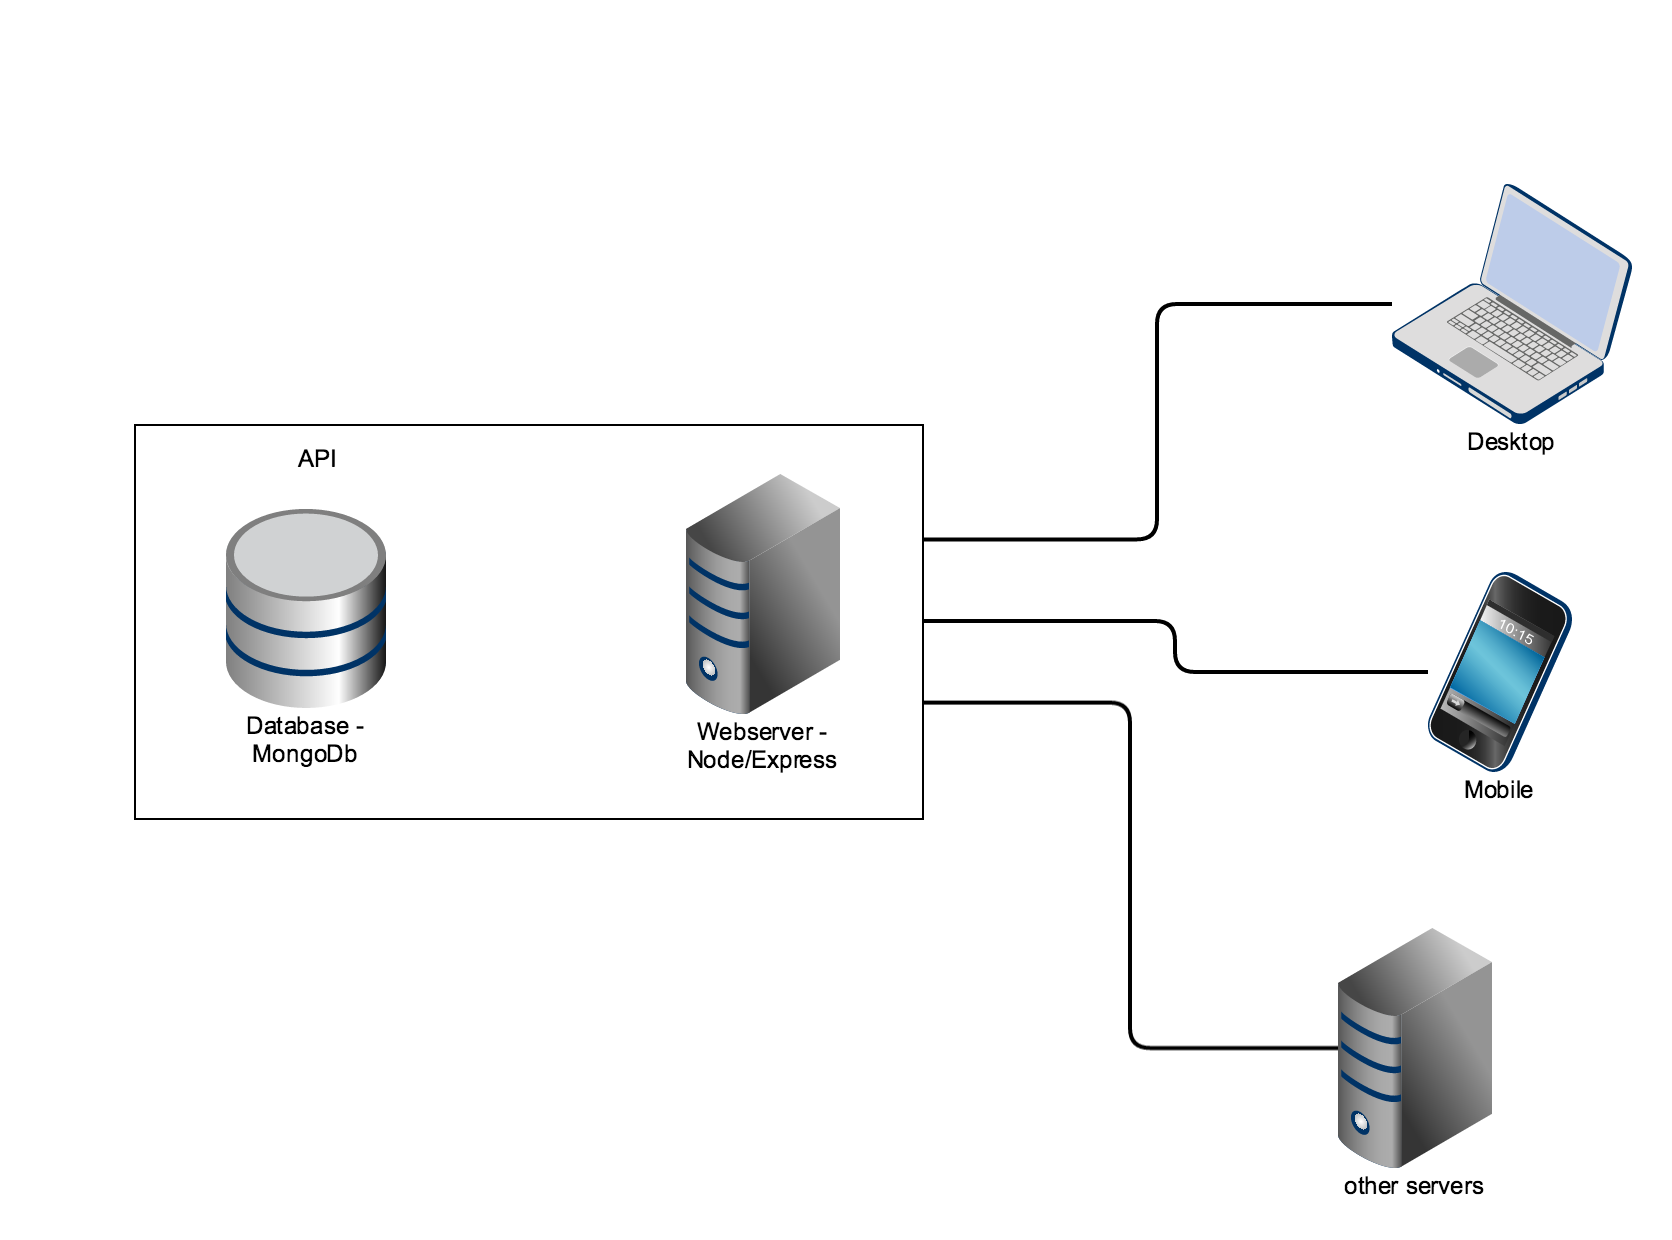
\includegraphics[width=\textwidth]{images/api_uses.png}

\subsection{Bootstrapping ExpressJS}

After a detour in the land of Node, MongoDB, Mongoose, and middleware,
we are back to our express \verb!todoApp! application. This time we will create the routes and
finalise our RESTful API.

Express has a separate package called \texttt{express-generator}, which
can help us to get started with out API.
\begin{Verbatim}
# install it globally using -g
npm install express-generator -g

# create todo-app API with EJS views (instead the default Jade)
express todo-api -e

#   create : todo-api
#   create : todo-api/package.json
#   create : todo-api/app.js
#   create : todo-api/public
#   create : todo-api/public/javascripts
#   create : todo-api/routes
#   create : todo-api/routes/index.js
#   create : todo-api/routes/users.js
#   create : todo-api/public/stylesheets
#   create : todo-api/public/stylesheets/style.css
#   create : todo-api/views
#   create : todo-api/views/index.ejs
#   create : todo-api/views/layout.ejs
#   create : todo-api/views/error.ejs
#   create : todo-api/public/images
#   create : todo-api/bin
#   create : todo-api/bin/www
#
#   install dependencies:
#     $ cd todo-api && npm install
#
#   run the app:
#     $ DEBUG=todo-app:* npm start
\end{Verbatim}
This will create a new folder called \texttt{todo-api}. Let's go ahead
and install the dependencies and run the app:
\begin{Verbatim}
# install dependencies
cd todo-api && npm install
# run the app
npm start
\end{Verbatim}
Use your browser to go to \url{http://0.0.0.0:3000}, and you should see
a message 
\begin{Verbatim}
	Welcome to Express.
\end{Verbatim}

\subsection{Connect ExpressJS to MongoDB}

In this section we are going to access MongoDB using our newly created
express app. Hopefully, you have installed MongoDB in the
setup section, and you can start it by typing (if you haven't yet):
\begin{Verbatim}
mongod
\end{Verbatim}
Install the MongoDB driver for NodeJS called mongoose:
\begin{Verbatim}
npm install mongoose --save
\end{Verbatim}
Notice \texttt{-\/-save}. It will add it to the \texttt{todo-api/package.json}

Next, you need to require mongoose in the \texttt{todo-api/app.js}
\begin{Verbatim}
// load mongoose package
var mongoose = require('mongoose');
// Use native Node promises
mongoose.Promise = global.Promise;
// connect to MongoDB
mongoose.connect('mongodb://localhost/todo-api')  
	.then(() =>  console.log('connection succesful'))  
	.catch((err) => console.error(err));
\end{Verbatim}
Now, when you run \texttt{npm\ start} or \texttt{./bin/www}, you will
(hopefully) see the message \texttt{connection\ successful}. 

\subsection{Creating the Todo model with Mongoose}

Create a \texttt{models} directory and a \texttt{Todo.js} model:
\begin{Verbatim}
mkdir models
touch models/Todo.js
\end{Verbatim}
In the \texttt{models/Todo.js}:
\begin{Verbatim}
var mongoose = require('mongoose');
var TodoSchema = new mongoose.Schema({  
	name: String,  
	completed: Boolean,  
	note: String,  
	updated_at: { type: Date, default: Date.now },});

module.exports = mongoose.model('Todo', TodoSchema);
\end{Verbatim}
You may well ask what this is about as MongoDB is supposed to be a schemaless database system?
Well, it is schemaless and flexible however, very often we want
validation and constraints in our API and therefore enforcing a
schema keeps the structure consistent; Mongoose does that for us.
You can use the following types:
\begin{itemize}
\item
  \verb!String!
\item
  \verb!Boolean!
\item
  \verb!Date!
\item
  \verb!Array!
\item
  \verb!Number!
\item
  \verb!ObjectId!
\item
  \verb!Mixed!
\item
  \verb!Buffer!
\end{itemize}

\section{API clients (Browser, Postman and curl)}

A slight aside now. Here are some tools which may prove useful in allowing easy
retrieve, change and delete data operations from your future API.

\subsection{Curl}

\begin{Verbatim}
# Create task
curl -XPOST http://localhost:3000/todos -d 'name=Master%20Routes&completed=false&note=soon...'
# List tasks
curl -XGET http://localhost:3000/todos
\end{Verbatim}

\subsection{Browser and Postman}

If you open your browser and type \texttt{localhost:3000/todos} you will
see all the tasks (when you implement it). However, you cannot do post
commands by default. For further testing let's use a Chrome plugin
called
\href{https://chrome.google.com/webstore/detail/postman-rest-client/fdmmgilgnpjigdojojpjoooidkmcomcm?hl=en}{Postman} (there is also a standalone app 
for those of you who prefer another browser option).
It allows you to use all the HTTP VERBS easily and check
\texttt{x-www-form-urlencoded} for adding parameters.

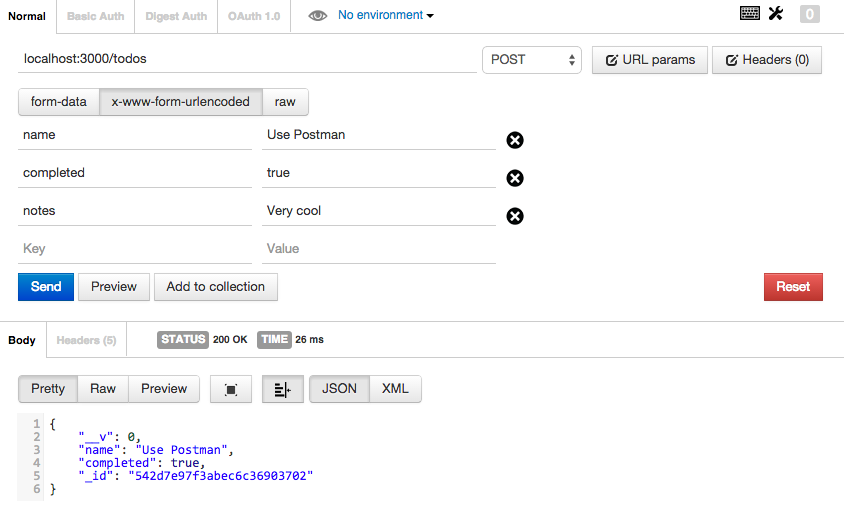
\includegraphics[width=\textwidth]{images/postman_post.png}

Don't forget to ``tick'' \texttt{x-www-form-urlencoded} or it won't work!

\subsection{Websites and Mobile Apps}

Probably these are the main consumers of APIs. You can interact with
RESTful APIs using jQuery's \texttt{\$ajax} and its wrappers,
BackboneJS's Collections/models, AngularJS's \texttt{\$http} or
\texttt{\$resource}, among many other libraries/frameworks and mobile
clients.

\section{ExpressJS Routes}

We want to achieve the following:
\begin{longtable}[]{@{}lllll@{}}
\toprule
Resource (URI) & POST (create) & GET (read) & PUT (update) & DELETE
(destroy)\tabularnewline
\midrule
\endhead
/todos & create new task & list tasks & error & error\tabularnewline
/todos/:id & error & show task :id & update task :id & destroy task ID
1\tabularnewline
\bottomrule
\end{longtable}
\noindent Let's setup the routes.
We'll create a new route called \verb!todos.js! in the \verb!routes! folder or rename
\verb!users.js!.
\begin{Verbatim}
mv routes/users.js routes/todos.js
\end{Verbatim}
In \texttt{app.js} add new \texttt{todos} route, or just replace
\texttt{./routes/users} for \texttt{./routes/todos}
\begin{Verbatim}
var todos = require('./routes/todos');
app.use('/todos', todos);
\end{Verbatim}
Edit the \texttt{routes/todos.js} file.

\subsection{List: GET /todos}

Remember the mongoose query api? Here's how to use it in this context:
\begin{Verbatim}
var express = require('express');
var router = express.Router();
var mongoose = require('mongoose');
var Todo = require('../models/Todo.js');

/* GET /todos listing. */
router.get('/', function(req, res, next) {  
	Todo.find(function (err, todos) {    
		if (err) return next(err);    
		res.json(todos);  
	});
});

module.exports = router;
\end{Verbatim}
We don't have any tasks in the database at the moment but at least we verify it is working:
\begin{Verbatim}
# Start database
mongod

# Start Webserver (in another terminal tab)
npm start

# Test API (in another terminal tab)
curl localhost:3000/todos
# => []%
\end{Verbatim}
If it returns an empty array \verb![]! you are all set. If you get
errors, try going back and making sure you didn't forget anything.

\subsection{Create: POST /todos}

Back in \texttt{routes/todos.js}, we are going to add the ability to
create using \protect\hyperlink{mongoose-create}{mongoose create}. Can
you make it work before looking at the next example?
\begin{Verbatim}
/* POST /todos */
router.post('/', function(req, res, next) {  
	Todo.create(req.body, function (err, post) {    
		if (err) return next(err);    
		res.json(post);  
	});
});
\end{Verbatim}
A few things are worth mentioning here:
\begin{itemize}
\item
  We are using the \texttt{router.post} instead of \texttt{router.get}.
\item
  You have to stop and run the server again: \texttt{npm\ start}.
\end{itemize}
Every time you change a file you have to stop and start the web server.
Let's fix that using \texttt{nodemon} to refresh automatically:
\begin{Verbatim}
# install nodemon globally
npm install nodemon -g

# Run web server with nodemon
nodemon
\end{Verbatim}

\subsection{Show: GET /todos/:id}

This is straightforward with
\texttt{Todo.findById} and
\texttt{req.params}. Notice that \texttt{params} matches the placeholder
name we set while defining the route. \texttt{:id} in this case.
\begin{Verbatim}
/* GET /todos/id */
router.get('/:id', function(req, res, next) {  
	Todo.findById(req.params.id, function (err, post) {    
		if (err) return next(err);    
		res.json(post);  
	});
});
\end{Verbatim}
Let's test what we have so far!
\begin{Verbatim}
# Start Web Server
nodemon

# Create a todo using the API
curl -XPOST http://localhost:3000/todos -d 
	'name=Master%20Routes&completed=false&note=soon...'
# => {"__v":0,"name":"Master Routes","completed":false,"note":"soon...","_id":"..."}%

# Get todo by ID (use the _id from the previous request)
curl -XGET http://localhost:3000/todos/
	57a655997d2241695585ecf8{"_id":"57a655997d2241695585ecf8","name":"Master 
	Routes","completed":false,"note":"soon...","__v":0}%

# Get all elements (notice it is an array)
curl -XGET http://localhost:3000/todos[{"_id":"57a655997d2241695585ecf8",
	"name":"Master Routes","completed":false,"note":"soon...","__v":0}]%
\end{Verbatim}

\subsection{Update: PUT /todos/:id}

Back in \texttt{routes/todos.js}, we are going to update tasks. 
\begin{Verbatim}
/* PUT /todos/:id */
router.put('/:id', function(req, res, next) {  
	Todo.findByIdAndUpdate(req.params.id, req.body, function (err, post) {    
		if (err) return next(err);    
		res.json(post);  
	});
});
\end{Verbatim}
Using curl:
\begin{Verbatim}
# Use the ID from the todo, in my case 57a655997d2241695585ecf8
curl -XPUT http://localhost:3000/todos/57a655997d2241695585ecf8 -d "note=hola"
# => {"_id":"57a655997d2241695585ecf8",
	"name":"Master Routes","completed":true,"note":"hola","__v":0}%
\end{Verbatim}

\subsection{Destroy: DELETE /todos/:id}

Almost identical to \texttt{update}, use
\texttt{findByIdAndRemove}.
\begin{Verbatim}
/* DELETE /todos/:id */
router.delete('/:id', function(req, res, next) {  
	Todo.findByIdAndRemove(req.params.id, req.body, function (err, post) {    
		if (err) return next(err);    
		res.json(post);  
	});
});
\end{Verbatim}

\section*{Acknowledgements}

This document is based upon an article by Adrian Mejia \url{http://adrianmejia.com}.
\end{document}